\newpage
\section{The Path Not Taken}
                                  

In Euclidean geometry, there is a unique shortest path between two
points. Not so in city geometry, here you have many different
choices. Let's investigate this further.


\begin{prob} 
Place two points $5$ units apart on the grid below. How many paths are
there that follow the grid lines? Note, if your answer is $1$, then
maybe you should pick another point!
\[
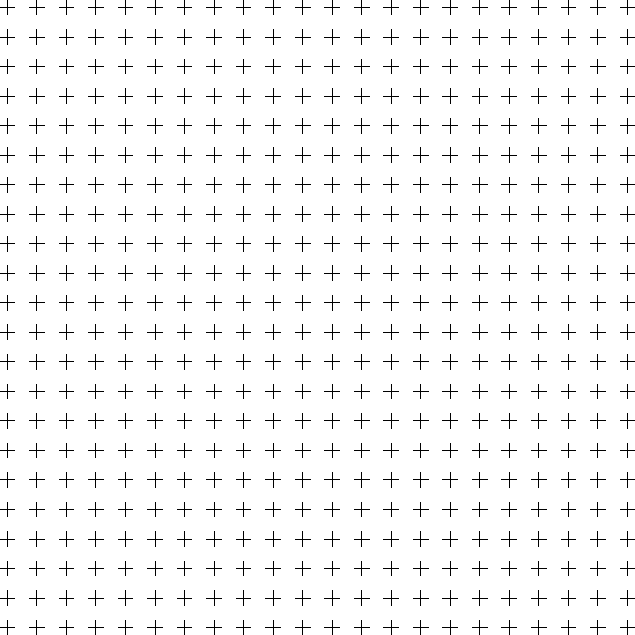
\includegraphics{../graphics/complexPlane}
\]
Be sure to demand that your results are shared with the rest of the
class.
\end{prob}

\begin{prob}
Do the first problem again, except for points that are 4 units apart
and then for points that are 6 units apart. What do you notice? Can
you explain this?
\end{prob}

\begin{prob}
Construct a chart showing your findings from your work above, and
other findings that may be relevant.
\end{prob}

\begin{prob}
Suppose you know how many paths there are to all points of distance
$n$ away from a given point. Can you easily figure out how many paths
there are to all points of distance $n+1$ away? Try to explain this in
the context of paths in city geometry.
\end{prob}
